\chapter{Технологический раздел}


\section{Выбор языка программирования}

В качестве языка программирования был выбран C++, так как на нем написана серверная часть базы данных MongoDB. Соответственно, метод хранения аудио-файлов для MongoDB был разработан, как патч для действующей версии СУБД.

\section{Выбор среды разработки}

Для программной реализации метода был выбран редактор кода Visual Studio Code \cite{VSC}, так как он обладает следующими достоинствами.
\begin{enumerate}
\item Кроссплатформенность.
\item Поддержка большого набора языков программирования, включая C++.
\item Широкие возможности кастомизации.
\item Открытый исходный код.
\end{enumerate}

\section{Выбор инструментов для замеров времени}

Для доступа к базе данных использовался драйвер C\# для MongoDB -- MongoDB.Driver \cite{CSDriver}, обеспечивающий асинхронное взаимодействие с MongoDB. MongoDB.Driver предоставляет API для подключения к серверу базы данных и выполнения запросов любой сложности через клиента. Такой подход наиболее удобен, когда планируется последующая программная обработка данных, как в случае с замером времени работы с данными при выбранном методе хранения.
Программное обеспечение было реализовано в интегрированной среде разработки Rider \cite{Rider}, которая является кроссплатформенной, предоставляет удобные и быстрые редактор кода и отладчик, поддерживает платформу .Net \cite{Net} для создания приложений на языке C\#, а также имеет свободный доступ для студентов. Установка драйвера была произведена с помощью пакетного менеджера NuGet \cite{NuGet}, имеющего удобный интерфейс в среде Rider, и была интегрирована в сборку проекта с помощью системы управления зависимостями .Net с указанием версии используемого пакета. На рис. 1.1 представлен фрагмент сборки приложения с драйвером MongoDB.Driver.

\begin{center}
		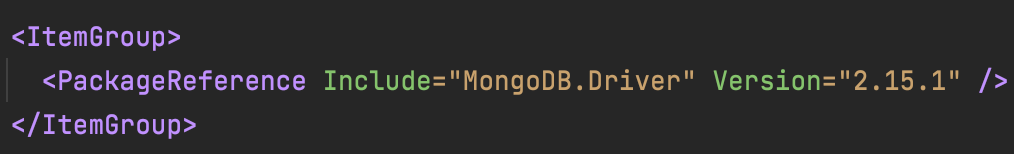
\includegraphics[scale=0.6]{img/MongoDriver}
		
			Рис 1.1 — Фрагмент сборки .Net приложения с интеграцией драйвера MongoDB.Driver 
\end{center} 

Для замеров времени работы реализованного метода при тестировании и сравнении его с аналогом хранения использовалась бибилиотека BenchmarkDotNet \cite{BenchMark}. BenchmarkDotNet - это легкая и мощная библиотека .NET с открытым исходным кодом, которая может преобразовывать методы в тесты, отслеживать эти методы, а затем предоставлять анализ полученных данных о производительности. BenchmarkDotNet обеспечивает высокую точность полученных результатов благодаря использованию набора инструментов для анализа производительности Perfolizer \cite{Perfolizer}. Широкий спектр возможностей, которые предоставляет данная библиотека, включает в себя анализ тестов, предупреждающий ошибки, и экспорт результатов сравнительного анализа методов в необходимом пользователю формате. Результатом запуска метода Run() данного инструмента со стандартной конфигурацией будет сводная таблица показателей производительности тестируемых методов.
BenchmarkDotNet была установлена в среду разработки так же с помощью менеджера пакетов NuGet и интегрирована в сборку проекта системой управления зависимостями. На рис. 1.2 представлен фрагмент сборки приложения с библиотекой BenchmarkDotNet.

\begin{center}
		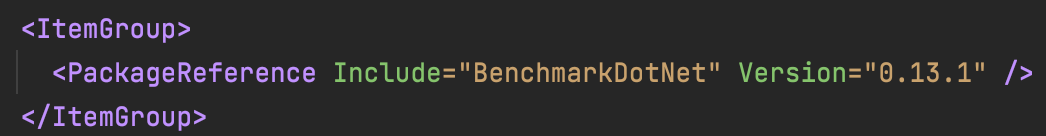
\includegraphics[scale=0.6]{img/BenchmarkDotNet}
		
			Рис 1.2 — Фрагмент сборки .Net приложения с интеграцией библиотеки BenchmarkDotNet 
\end{center} 

\section{Сборка локального сервера MongoDB}

Следуя инструкции по сборке MongoDB из исходного кода, расположенной в официальном репозитории базы данных \cite{Instruction}, для компиляции сервера MongoDB использовался инструмент для автоматизации сборки программных проектов SCons \cite{SCons}. Команда, использовавшаяся для запуска компиляции сервера MongoDB в командной строке с помощью SCons, представлена в листинге \ref{lst:scons_command}, где 
\begin{enumerate}
\item dbg -- вывод отладочной информации.
\item j8 -- количество логических ядер, между которыми распределяется нагрузка при компиляции (8).
\item install-mongod -- цель, указывающая какой компонент нужно скомпилировать.
\end{enumerate}

\begin{lstlisting}[language=sql, label=some-code, caption=Команда для компиляции сервера MongoDB средствами SCons, label=lst:scons_command]
sudo scons --dbg -j8 install-mongod  
\end{lstlisting}

Для сборки SCons использует скрипты SConstruct, расположенные в файловой структуре проекта, одними из задач которых является импортирование необходимых модулей Python и проверка инструментов, участвующих в компиляции, на соответствие требованиям.

Для успешной сборки определены следующие требования.

\begin{enumerate}
\item Современный С++ компилятор. Подходят следующие компиляторы.
\begin{enumerate}
\item G++ 8.2 \cite{GCC} или новее.
\item Clang 7.0 \cite{Clang} или новее.
\end{enumerate}
\item В операционных системах Linux \cite{Linux} и macOS \cite{macOS} требуется библиотека и заголовок libcurl \cite{LibCurl}. MacOS включает libcurl.
\item Python 3.7 и некоторые модули, устанавливаемые с помощью команды, представленной в листинге \ref{lst:python_modules}.
\item Около 13 ГБ свободного места на диске для скомпилированных двоичных файлов.
\end{enumerate}

\begin{lstlisting}[language=sql, label=some-code, caption=Команда для установки необходимых для сборки модулей Python, label=lst:python_modules]
python3 -m pip install -r etc/pip/compile-requirements.txt  
\end{lstlisting}

SCons также предоставляет возможность скомпилировать отдельные компоненты MongoDB, задав одну или несколько из следующих целей.
\begin{enumerate}
\item install-mongod -- сервер базы данных.
\item install-mongos -- шардинг.
\item install-servers -- включает install-mongod и install-mongos.
\item install-core -- включает install-mongod и install-mongos.
\item install-mongosh -- полнофукционольная среда для взаимодействия с развертываниями MongoDB, использующая интерфейс командной строки.
\item install-all -- все компоненты.
\end{enumerate}

\section{Структура проекта}

В проект базы данных MongoDB было добавлено два исходных файла, реализующих логику добавления и извлечения MIDI-файла, а также заголовочные файлы для них. 

Так как MIDI-файл, в соответствии с разработанным методом, хранится в виде предварительно распарсенной структуры, программный код, выполняющий считывание потока байтов из файла и конструирование из него документа, находится в части проекта, отвечающей за выполнение операции вставки в базу данных. На этапе валидирования добавляемого документа выполняется проверка на то, содержит ли он путь к MIDI-файлу, и если да -- документ пересобирается с использованием парсера, чтобы впоследствии представлять внутреннюю структуру аудио-файла.

В проект по пути src/mongo/db/ops/ были добавлены следующие файлы для парсинга MIDI-файла на этапе вставки документа в MongoDB.
\begin{enumerate}
\item insert\_midi.cpp -- исходный файл, реализующий чтение MIDI-файла и парсер.
\item insert\_midi.h -- заголовочный файл.
\end{enumerate}

Для дальнейшей работы с добавленным документом, как с аудио-файлом, предусмотрено обратное преобразование структуры в MIDI-файл в процессе извлечения документы из базы данных. Для этого добавлена проверка на то, что запись в MongoDB является MIDI-файлом, и последовательная запись данных в файл с именем, которое было указано пользователем в качестве второго поля при вставке аудио-файла (name) или, в случае если пользователь указал только путь к файлу, извлечено из пути.

В проект по пути src/mongo/db/commands/ были добавлены следующие файлы для воссоздания MIDI-файла на этапе извлечения документа из MongoDB.
\begin{enumerate}
\item find\_midi.cpp -- исходный файл, реализующий обратное преобразование документа в MIDI-файл.
\item find\_midi.h -- заголовочный файл.
\end{enumerate}

Для успешной сборки проекта после добавления новых файлов требуется указать их в конфигурации соответствующих файлов SConstruct. Следовательно, были изменены следующие скрипты.
\begin{enumerate}
\item src/mongo/db/SConscript.
\item src/mongo/db/commands/SConscript.
\end{enumerate}

\section{Пример работы реализованного метода}

Для демонстрации работы метода был создан клиент MongoDB на языке Python с помощью библиотеки pymongo \cite{PyMongo}. Помимо поддержки API доступа к MongoDB и работы с ней, Python предоставляет возможность загружать и проигрывать аудиозаписи различных форматов, как фоновую музыку, с использованием средств библиотеки pygame \cite{PyGame}. Также Python содержит бибилиотеку tkinter \cite{Tk}, с помощью которой был реализован простой графический интерфейс для удобства работы с базой данных.

Однако, независимо от используемого клиента, структура данных для запроса на добавление MIDI-файла в базу данных примет следующий вид (листинг \ref{lst:insert_command}).

\begin{lstlisting}[language=sql, label=some-code, caption=Данные для запроса на добавление MIDI-файла в MongoDB, label=lst:insert_command]
{path: "/Users/anastasia/Desktop/ProgramEngineering/some_audio.mid",  name:"my_audio"}
\end{lstlisting}

Для извлечения данных с последующим сохранением MIDI-файла с названием my \_audio достаточно установить в фильтре запроса на извлечение значение True поля MidiSave. Если не нужно сохранять аудио-файл локально, значение поля MidiSave в фильтре можно установить равным False или опустить.

На рисунке 1.3 представлен реализованный для демонстрации графический интерфейс.

\begin{center}
		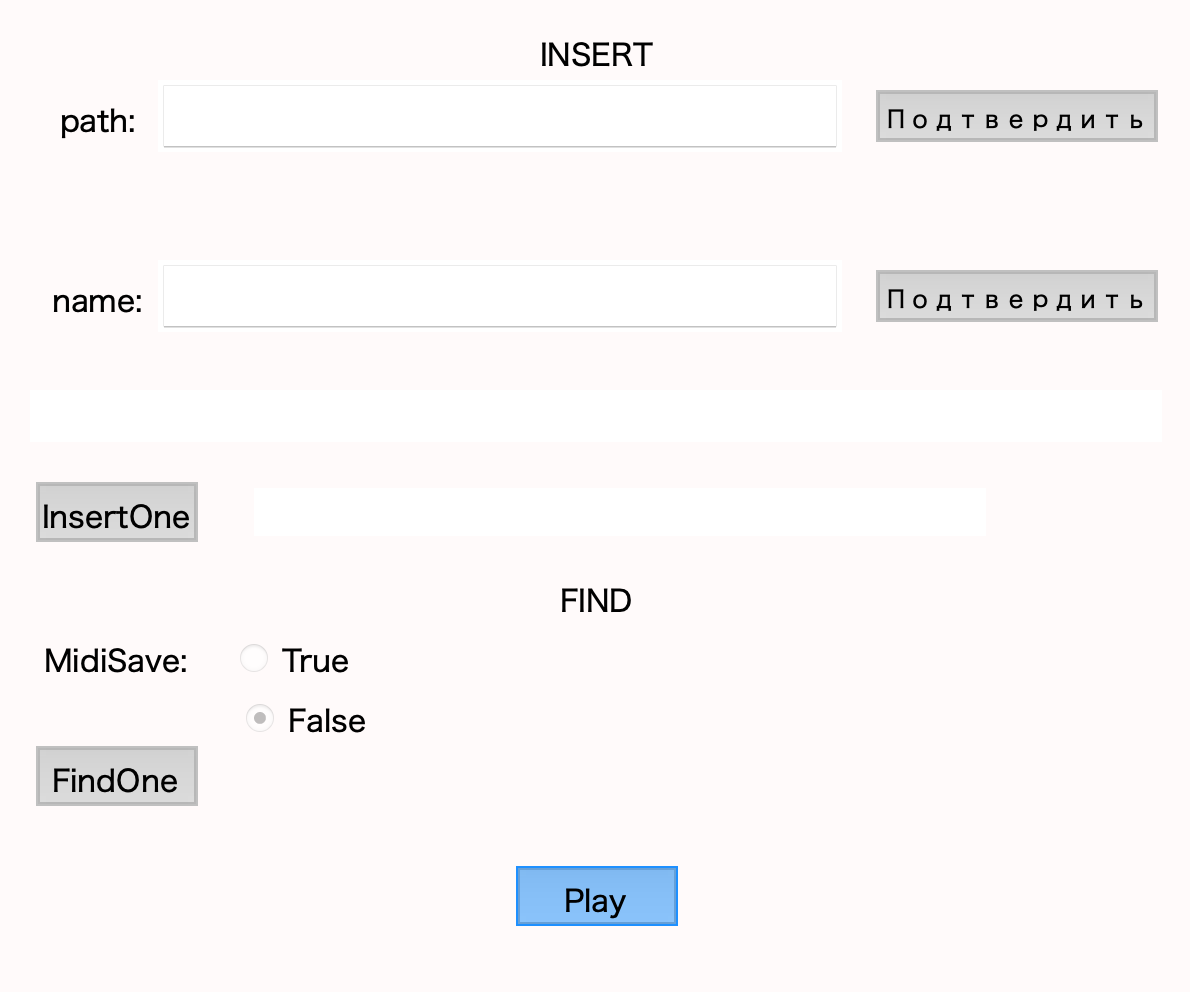
\includegraphics[scale=0.6]{tex/img/Tkinter.png}
		
			Рис 1.3 — Графический интерфейс для демонстрации работы метода
\end{center} 

После заполнения полей path и name будут сформированы данные для запроса к MongoDB на вставку, который бдует выполнен при нажатии на кнопку InsertOne. Результатом успешной операции является идентификатор добавленного в базу данных документа (рис. 1.4). 

\begin{center}
		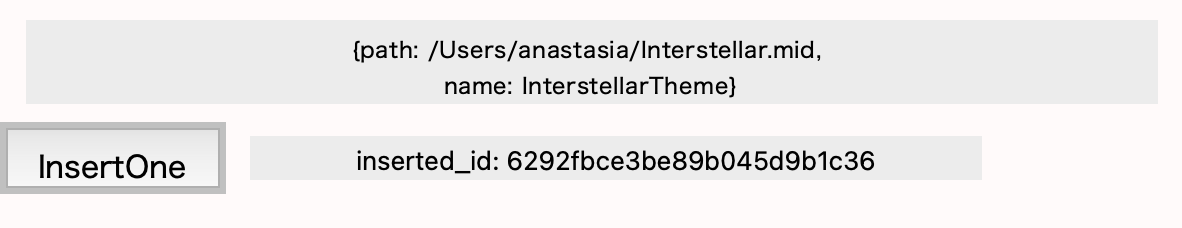
\includegraphics[scale=0.6]{tex/img/Tkinter1.png}
		
			Рис 1.4 — Результат успешного добавления MIDI-файла в MongoDB
\end{center} 

Для извлечения документа с сохранением MIDI-файла полю MidiSave устанавливается значение True. В таком случае документ, извлеченный из базы данных, будет сохранен локально, как файл MIDI с именем InterstellarTheme, который может быть воспроизведен с помощью кнопки Play.

Для удобного просмотра документа в базе данных можно также использовать команду mongosh (листинг \ref{lst:find_command}), где midiFiles -- это коллекция документов.

\begin{lstlisting}[language=sql, label=some-code, caption=Команда mongosh для просмотра документов в MongoDB, label=lst:find_command]
db.midiFiles.find()
\end{lstlisting}

Результатом выполнения этой команды будет вывод всех документов коллекции (в данном случае, одного только что добавленного документа, так как коллекция была пуста) в консоль (рис. 1.5 -- 1.6).

\begin{center}
		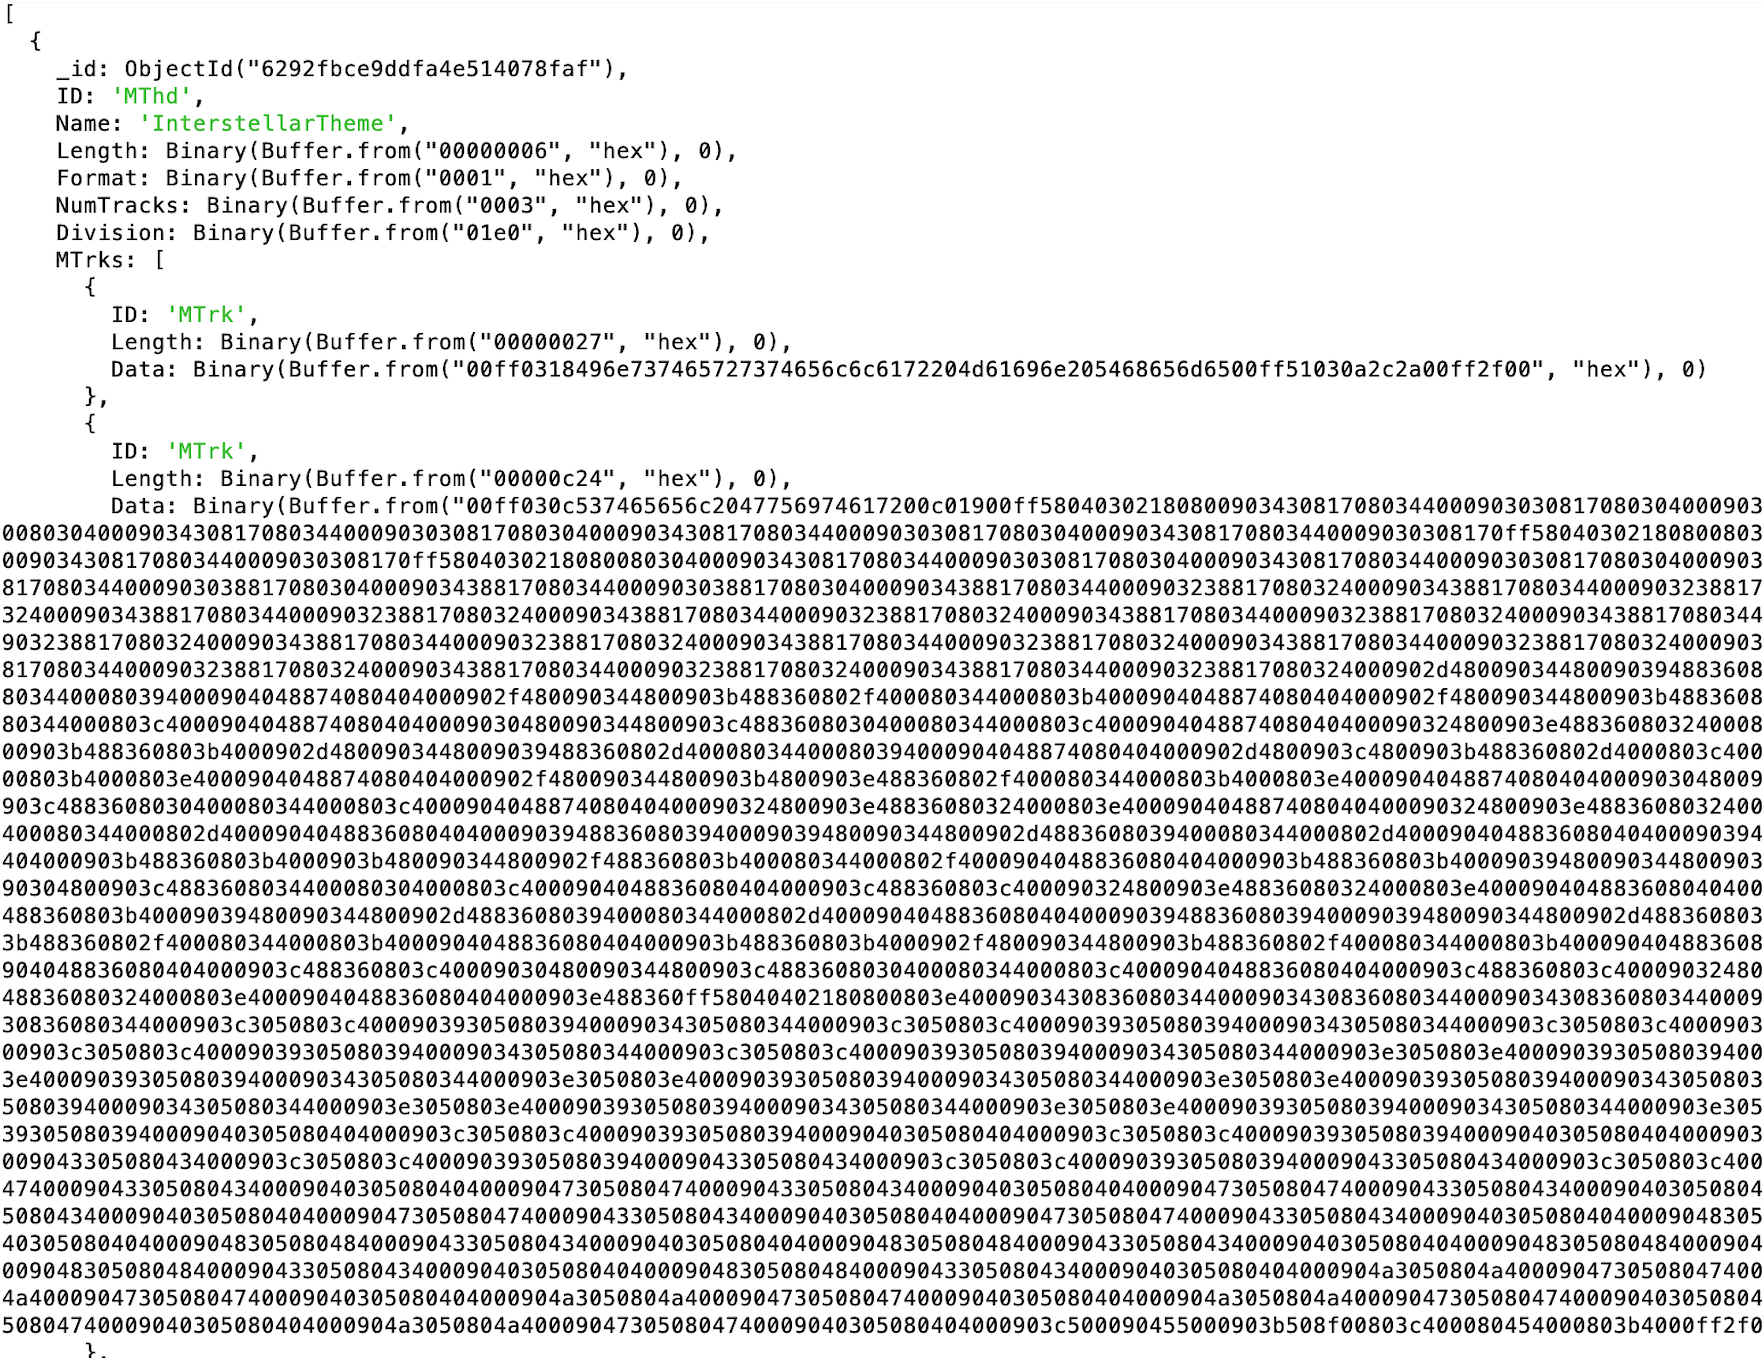
\includegraphics[scale=0.5]{tex/img/Console1.png}
		
			Рис 1.5 — Результат извлечения MIDI-файла из MongoDB (часть 1)
\end{center} 

\begin{center}
		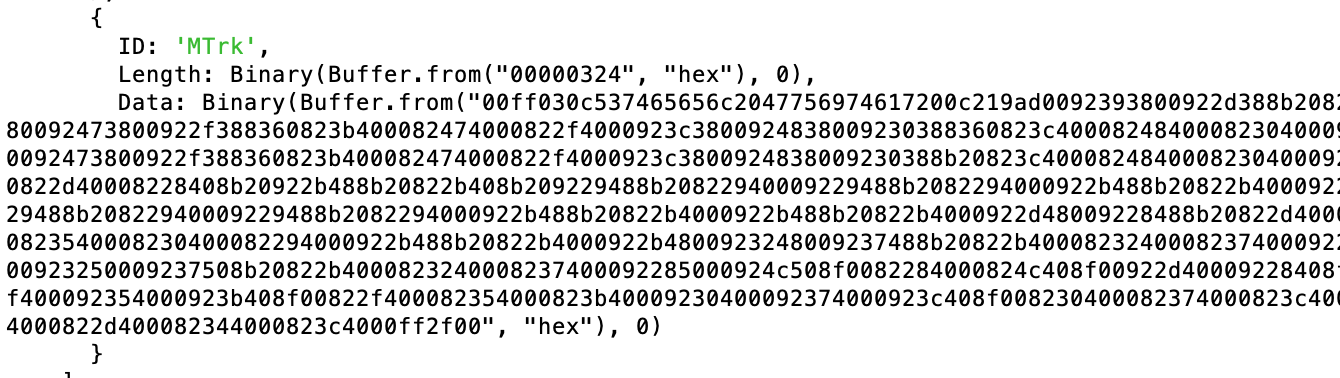
\includegraphics[scale=0.6]{tex/img/Console2.png}
		
			Рис 1.6 — Результат извлечения MIDI-файла из MongoDB (часть 2)
\end{center}


\section{Выводы из технологического раздела}

В данном разделе был обоснован выбор средств программной разработки метода хранения аудио-файлов в NoSQL-базе данных и вспомогательных инструментов для замера времени работы метода и демонстрации его работы. Также была приведена инструкция сборки проекта MongoDB с интегрированным методом и были описаны изменения его структуры. Было проведено тестирование метода с использованием графического интерфейса и интерфейса командной строки.